
%(BEGIN_QUESTION)
% Copyright 2008, Tony R. Kuphaldt, released under the Creative Commons Attribution License (v 1.0)
% This means you may do almost anything with this work of mine, so long as you give me proper credit

Examine the following graphs, plotting pressures along the fluid flow path within three different control valves:

$$\includegraphics[width=15.5cm]{i01418x01.eps}$$

As you can see from the graphs, the inlet pressures ($P_1$) and outlet pressures ($P_2$) are the same for each valve.  That is, each of the three valves exhibits the same amount of permanent pressure drop.  However, what happens inside each valve is quite different, an indicated by the different {\it vena contracta} pressures ($P_{vc}$).

When fluid enters a constricted portion of the valve, its velocity increases.  A greater fluid velocity means the fluid molecules possess greater kinetic energy than before.  In accordance with the Law of Energy Conservation, this increase in kinetic energy must be balanced by a corresponding loss in potential energy (fluid pressure) through the constriction.  This is what accounts for the sudden decrease in pressure at the vena contracta point (the point of maximum constriction inside the valve).  

After passing through the constriction, the fluid enters a wider portion of the valve and slows down.  Molecular kinetic energy decreases while potential energy (pressure) increases.  This is why pressure ``recovers'' downstream of the vena contracta.  The difference between upstream and downstream pressures ($P_1 - P_2$) represents fluid energy lost in the throttling action of the valve.

\vskip 10pt

Determine which of the three valves has the greatest {\it pressure recovery}, and which of the three valves has the greatest {\it pressure recovery factor} (sometimes referred to as {\it pressure recovery coefficient}).  Then, determine which of the three valves is more prone to cavitation in liquid service, all other factors being equal.

Finally, identify control valve types characterized by extremes of pressure recovery and pressure recovery factor.

\underbar{file i01418}
%(END_QUESTION)





%(BEGIN_ANSWER)

{\it Pressure recovery} is the pressure difference between the outlet pressure ($P_2$) and vena contracta pressure ($P_{vc}$):

$$\hbox{Pressure recovery} = P_2 - P_{vc}$$

$$\includegraphics[width=15.5cm]{i01418x02.eps}$$

{\it Pressure recovery factor} is calculated by dividing the permanent pressure drop by the pressure drop from inlet ($P_1$) to the vena contracta ($P_{vc}$):

$$F_L = \sqrt{{P_1 - P_2} \over {P_1 - P_{vc}}}$$

Based on this definition, valve \#1 has the greatest pressure recovery and the lowest $F_L$, making it the most prone to cavitation.  To avoid or reduce cavitation, it is best to use a control valve with low pressure recovery (a high $F_{L}$ factor).  Rotary valve designs such as ball, disk, and butterfly valves typically have greater pressure recovery (lower $F_{L}$ figures) than globe valves, making them more prone to cavitation.

\vskip 10pt

Ironically, control valves with low pressure recovery have high $F_L$ values.  Conversely, valves with high pressure recovery have low $F_L$ values.  To avoid or reduce cavitation, it is best to use a control valve with low pressure recovery (a large $F_{L}$ factor).  All other factors being equal (upstream and downstream pressures, flow rate, specific gravity, etc.), a valve with a large $F_{L}$ will have a greater vena contracta pressure ($P_{vc}$) than a valve with a small $F_{L}$.

\vskip 10pt

Rotary valve designs (ball, disk, butterfly, etc.) typically have greater pressure recovery (smaller $F_{L}$ figures) than globe valves, making them more prone to cavitation.  The reason for this greater pressure recovery is the relatively straight and wide flow path through a rotary valve body before and after the throttling element.  Globe valves, with their more tortuous flow paths, drop more pressure along the whole valve body.  As a result, the plug/seat opening in a globe valve does not have to do {\it all} the work of dropping process fluid pressure.

For the same total pressure drop ($P_1 - P_2$), a globe valve's trim will drop less pressure than a rotary valve's trim of comparable $C_{v}$.  This results in a greater vena contracta pressure ($P_{vc}$) inside the globe valve, making is less prone to flashing and cavitation than a comparable rotary valve.

\filbreak

The following illustration shows the difference in flow paths between a butterfly valve and a globe valve.  You can see here how the globe valve design does not rely on the plug/seat restriction to be the {\it only} point of pressure drop as is the case with the butterfly design:
 
$$\includegraphics[width=15.5cm]{i01418x03.eps}$$

\vskip 10pt

$F_L$ changes with valve stem position, just like $C_v$.  For high-$F_L$ valves such as globe valves, the amount of $F_L$ change throughout the valve's travel is slight.  For low-$F_L$ valves such as butterfly valves, the amount of $F_L$ change is much greater from fully open to fully shut.

\vskip 10pt

Valve trim designed to reduce cavitation typically achieves very high (near-unity) $F_L$ values.  For Fisher's Cavitrol trim, the advertised $F_L$ value for two-stage trim is 0.98, and for three-stage trim it is 0.99, which means $P_{vc}$ is very nearly equal to $P_2$ (downstream).

\vskip 10pt

\filbreak

Follow-up question: examine the following illustrations and then explain {\it why} rotary valve designs such as butterfly and ball valves tend to have lower $F_L$ values than comparably-sized globe valves:

$$\includegraphics[width=15.5cm]{i01418x03.eps}$$

%(END_ANSWER)





%(BEGIN_NOTES)


%INDEX% Final Control Elements, valve: cavitation control
%INDEX% Final Control Elements, valve: pressure recovery coefficient
%INDEX% Final Control Elements, valve: pressure recovery factor

%(END_NOTES)


